%!Tex Root = ../Main.tex
% ./Packete_und_Deklarationen.tex
% ./Titlepage.tex
% ./Motivation.tex
% ./Einführung.tex
% ./Implementierung2.tex
% ./Ergebnisse_und_Ausblick.tex

\chapter{Implementierung}
\label{ch:implementierung}
\section{Architektur}
% Unterscheid zur Architektur aus dem Bachelorprojekt

% Cross Compiler
% https://tex.stackexchange.com/questions/8625/force-figure-placement-in-text
\begin{figure}[H]
  \centering
  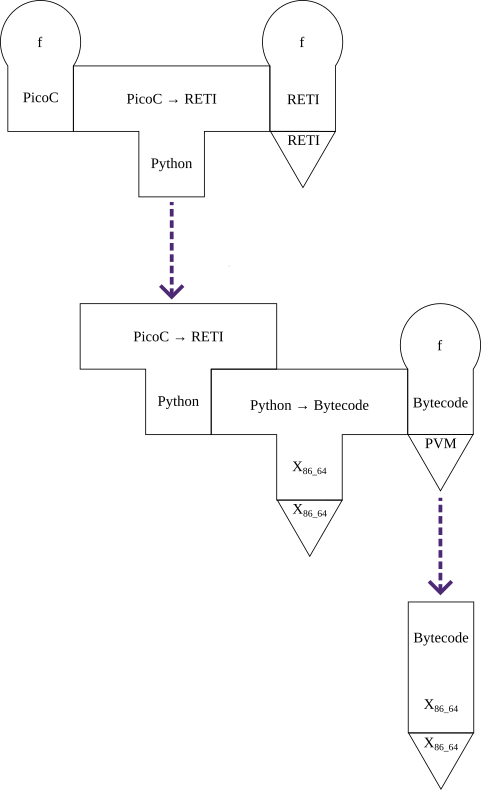
\includegraphics[width=0.5\linewidth]{./figures/summarized_cross_compiler.png}
  \caption{Cross-Compiler Kompiliervorgang ausgeschrieben}
\end{figure}

\begin{figure}[H]
  \centering
  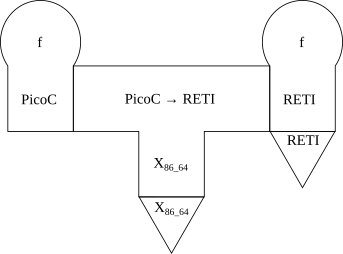
\includegraphics[width=0.33\linewidth]{./figures/compiliervorang_mit_machiene.png}
  \caption{Cross-Compiler Kompiliervorgang Kurzform}
\end{figure}

\begin{figure}[H]
  \centering
  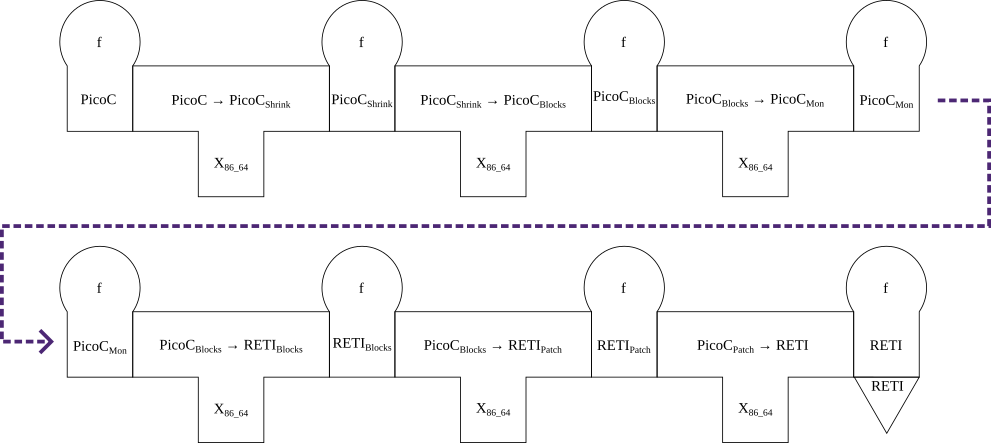
\includegraphics[width=\linewidth]{./figures/passes.png}
  \caption{Architektur mit allen Passes ausgeschrieben}
\end{figure}

\section{Lexikalische Analyse}
\subsection{Verwendung von Lark}
\numberwithin{floatgrammar}{section}

\label{sec:lex_analyse_verwendung_von_lark}
% ./concrete_syntax_picoc.lark
\begin{grammar}[Konkrette Syntax des Lexers][H][gr:concrete_syntax_lex]
  \toprule
  \firstcase{COMMENT}{\dq //\dq\enspace /[{\wedge}\backslash n]{*}/\gralt \dq {/*}\dq\enspace  /(.\mid \setminus n)*?/\enspace \dq {*/}\dq }{L\_Comment}
  \firstcase{RETI\_COMMENT.2}{\dq {//}\dq \dq \text{\textvisiblespace} \dq ? \dq \#\dq /[\wedge\backslash n]{*}/}{}
  \midrule
  \firstcase{DIG\_NO\_0}{\dq 1\dq \gralt \dq 2\dq \gralt \dq 3\dq \gralt \dq 4\dq \gralt \dq 5\dq}{L\_Arith}
  \otherform{\dq 6\dq \gralt \dq 7\dq \gralt \dq 8\dq \gralt \dq 9\dq}{}
  \firstcase{DIG\_WITH\_0}{\dq 0\dq \gralt DIG\_NO\_0}{}
  \firstcase{NUM}{\dq 0\dq \gralt DIG\_NO\_0 DIG\_WITH\_0*}{}
  \firstcase{ASCII\_CHAR}{\dq\text{\textvisiblespace} \dq ..\dq \sim\dq }{}
  \firstcase{CHAR}{\dq '\dq ASCII\_CHAR\dq '\dq }{}
  \firstcase{FILENAME}{ASCII\_CHAR+\dq .picoc\dq }{}
  \firstcase{LETTER}{\dq {a}\dq ..\dq {z}\dq \gralt \dq {A}\dq ..\dq {Z}\dq}{}
  \firstcase{NAME}{(LETTER\gralt \dq \_\dq )}{}
  & & (LETTER\gralt DIG\_WITH\_0\gralt \dq \_\dq )* & \\
  \firstcase{name}{NAME\gralt INT\_NAME\gralt CHAR\_NAME}{}
  \otherform{VOID\_NAME}{}
  \firstcase{NOT}{\dq \sim\dq }{}
  \firstcase{REF\_AND}{\dq \&\dq }{}
  \firstcase{un\_op}{SUB\_MINUS\gralt LOGIC\_NOT\gralt NOT}{}
  \otherform{MUL\_DEREF\_PNTR \gralt REF\_AND}{}
  \firstcase{MUL\_DEREF\_PNTR}{\dq {*}\dq }{}
  \firstcase{DIV}{\dq /\dq }{}
  \firstcase{MOD}{\dq \%\dq }{}
  \firstcase{prec1\_op}{MUL\_DEREF\_PNTR\gralt DIV\gralt MOD}{}
  \firstcase{ADD}{\dq {+}\dq }{}
  \firstcase{SUB\_MINUS}{\dq {-}\dq }{}
  \firstcase{prec2\_op}{ADD\gralt SUB\_MINUS}{}
  \midrule
  \firstcase{LT}{\dq {<}\dq }{L\_Logic}
  \firstcase{LTE}{\dq {<=}\dq }{}
  \firstcase{GT}{\dq {>}\dq }{}
  \firstcase{GTE}{\dq {>=}\dq }{}
  \firstcase{rel\_op}{LT\gralt LTE\gralt GT\gralt GTE}{}
  \firstcase{EQ}{\dq {==}\dq }{}
  \firstcase{NEQ}{\dq {!=}\dq }{}
  \firstcase{eq\_op}{EQ\gralt NEQ}{}
  \firstcase{LOGIC\_NOT}{\dq !\dq }{}
  \midrule
  \firstcase{INT\_DT.2}{\dq int\dq }{}
  \firstcase{INT\_NAME.3}{\dq int\dq\enspace (LETTER\gralt DIG\_WITH\_0\gralt \dq \_\dq )+}{L\_Assign\_Alloc}
  \firstcase{CHAR\_DT.2}{\dq char\dq }{}
  \firstcase{CHAR\_NAME.3}{\dq char\dq\enspace (LETTER\gralt DIG\_WITH\_0\gralt \dq \_\dq )+}{}
  \firstcase{VOID\_DT.2}{\dq void\dq }{}
  \firstcase{VOID\_NAME.3}{\dq void\dq\enspace (LETTER\gralt DIG\_WITH\_0\gralt \dq \_\dq )+}{}
  \firstcase{prim\_dt}{INT\_DT\gralt CHAR\_DT\gralt VOID\_DT}{}
  \bottomrule
\end{grammar}

\begin{grammar}[\(\lambda\) calculus syntax][p][gr:ex1]
	\firstcase{T}{\nonterm{V}}{Variable}
	\otherform{(\nonterm{T}\ \nonterm{T})}{Application}
	\otherform{\lambda \nonterm{V}\cdot\nonterm{T}}{Abstraction}
	\firstcase{V}{x, y, \dots}{Variables}
\end{grammar}
\begin{grammar}[Advanced capabilities of \texttt{grammar.sty}][p][gr:ex2]
	\firstcase{A}{\nonterm{T} \gralt \nonterm{V}}{Multiple option on a single line}
	\highlight
	\otherform{\nonterm{A}}{Highlighted form}
	\downplay
	\otherform{\nonterm{B}\gralt \nonterm{C}}{Downplayed form}
	\otherform{\lochighlight{\nonterm{A}} \gralt \nonterm{B}}{Emphasize part of the line}
\end{grammar}

% erwähnen, dass in Lark die Grammatiken L_Lex und L_Parse gemischt sind
% EBNF erwähnen
% (erwähnen, dass finalle Grammatik im Appendix)
\subsection{Basic Parser}
\section{Syntaktische Analyse}
\subsection{Verwendung von Lark}
% ./concrete_syntax_picoc.lark
% https://tex.stackexchange.com/questions/851/removing-spaces-between-words-in-math-mode
In \ref{gr:concrete_syntax_parser}

\begin{grammar}[Konkrette Syntax des Parsers, Teil 1][H][gr:concrete_syntax_parser]
  \toprule
	\downplay
  \firstcase{prim\_exp}{name\gralt NUM\gralt CHAR\gralt "("logic\_or")"}{L\_Arith +}
	\downplay
  \firstcase{post\_exp}{array\_subscr\gralt struct\_attr\gralt fun\_call}{L\_Array +}
	\downplay
  \otherform{input\_exp\gralt print\_exp\gralt prim\_exp}{L\_Pntr +}
	\downplay
  \firstcase{un\_exp}{un\_op un\_exp\gralt post\_exp}{L\_Struct + L\_Fun}
  \midrule
	\downplay
  \firstcase{input\_exp}{\dq input\dq\dq(\dq\dq)\dq}{L\_Arith}
	\downplay
  \firstcase{print\_exp}{\dq print\dq\dq(\dq logic\_or\dq)\dq}{}
	\downplay
  \firstcase{arith\_prec1}{arith\_prec1\enspace prec1\_op\enspace un\_exp\gralt un\_exp}{}
	\downplay
  \firstcase{arith\_prec2}{arith\_prec2\enspace prec2\_op\enspace arith\_prec1\gralt arith\_prec1}{}
	\downplay
  \firstcase{arith\_and}{arith\_and\enspace \dq\&\dq\enspace arith\_prec2\gralt arith\_prec2}{}
	\downplay
  \firstcase{arith\_oplus}{arith\_oplus\enspace \dq {\wedge{}}\dq\enspace arith\_and\gralt arith\_and}{}
	\downplay
  \firstcase{arith\_or}{arith\_or\enspace \dq{\mid} \dq\enspace arith\_oplus\gralt arith\_oplus}{}
  \midrule
  \downplay
  \firstcase{rel\_exp}{rel\_exp\enspace rel\_op\enspace arith\_or\gralt arith\_or}{L\_Logic}
  \downplay
  \firstcase{eq\_exp}{eq\_exp\enspace eq\_op rel\_exp\gralt rel\_exp}{}
  \downplay
  \firstcase{logic\_and}{logic\_and\enspace \dq{\&\&}\dq\enspace eq\_exp\gralt eq\_exp}{}
  \downplay
  \firstcase{logic\_or}{logic\_or\enspace \dq{\mid\mid}\dq\enspace logic\_and\gralt logic\_and}{}
  \midrule
	\downplay
  \firstcase{type\_spec}{prim\_dt\gralt struct\_spec}{L\_Assign\_Alloc}
	\downplay
  \firstcase{alloc}{type\_spec\enspace pntr\_decl}{}
	\downplay
  \firstcase{assign\_stmt}{un\_exp\enspace \dq {=}\dq\enspace logic\_or\dq ;\dq }{}
  \firstcase{initializer}{logic\_or\gralt array\_init\gralt struct\_init}{}
	\downplay
  \firstcase{init\_stmt}{alloc\enspace \dq {=}\dq\enspace initializer\dq ;\dq }{}
	\downplay
  \firstcase{const\_init\_stmt}{\dq const\dq\enspace type\_spec\enspace name\enspace \dq {=}\dq\enspace NUM\dq ;\dq }{}
  \midrule
  \firstcase{pntr\_deg}{\dq {*}\dq *}{L\_Pntr}
  \firstcase{pntr\_decl}{pntr\_deg\enspace array\_decl\gralt array\_decl}{}
  \midrule
  \firstcase{array\_dims}{(\dq [\dq NUM\dq ]\dq )*}{L\_Array}
  \firstcase{array\_decl}{name\enspace array\_dims\gralt \dq (\dq pntr\_decl\dq )\dq  array\_dims}{}
  \firstcase{array\_init}{\dq \{\dq initializer(\dq ,\dq\enspace initializer)*\dq \}\dq }{}
  \firstcase{array\_subscr}{post\_exp\dq [\dq logic\_or\dq ]\dq }{}
  \midrule
  \firstcase{struct\_spec}{\dq struct\dq\enspace name}{L\_Struct}
  \firstcase{struct\_params}{(alloc\dq ;\dq )+}{}
  \firstcase{struct\_decl}{\dq struct\dq\enspace name\enspace \dq \{\dq struct\_params\dq \}\dq }{}
  \firstcase{struct\_init}{\dq \{\dq \dq .\dq name\dq {=}\dq initializer}{}
  & & (\dq ,\dq\enspace \dq .\dq name\dq {=}\dq initializer)*\dq \}\dq & \\
  \firstcase{struct\_attr}{post\_exp\dq .\dq name}{}
  \midrule
	\downplay
  \firstcase{if\_stmt}{\dq if\dq \dq (\dq logic\_or\dq )\dq\enspace exec\_part}{L\_If\_Else}
	\downplay
  \firstcase{if\_else\_stmt}{\dq if\dq \dq (\dq logic\_or\dq )\dq\enspace exec\_part\enspace \dq else\dq\enspace exec\_part}{}
  \midrule
	\downplay
  \firstcase{while\_stmt}{\dq while\dq \dq (\dq logic\_or\dq )\dq\enspace exec\_part}{L\_Loop}
	\downplay
  \firstcase{do\_while\_stmt}{\dq do\dq\enspace exec\_part\enspace \dq while \dq \dq (\dq logic\_or\dq )\dq \dq ;\dq }{}
  \bottomrule
\end{grammar}

\begin{grammar}[Konkrette Syntax des Parsers, Teil 2][H]
  \toprule
	\downplay
  \firstcase{decl\_exp\_stmt}{alloc\dq ;\dq }{L\_Stmt}
	\downplay
  \firstcase{decl\_direct\_stmt}{ assign\_stmt\gralt init\_stmt\gralt const\_init\_stmt}{}
  \firstcase{decl\_part}{ decl\_exp\_stmt\gralt decl\_direct\_stmt\gralt RETI\_COMMENT}{}
  \\[-0.2cm]
	\downplay
  \firstcase{compound\_stmt}{ \dq \{\dq exec\_part* \dq \}\dq }{}
	\downplay
  \firstcase{exec\_exp\_stmt}{logic\_or\dq ;\dq }{}
	\downplay
  \firstcase{exec\_direct\_stmt}{if\_stmt\gralt if\_else\_stmt\gralt while\_stmt\gralt do\_while\_stmt}{}
	\downplay
  \otherform{assign\_stmt\gralt fun\_return\_stmt}{}
  \firstcase{exec\_part}{compound\_stmt\gralt exec\_exp\_stmt\gralt exec\_direct\_stmt}{}
  \otherform{RETI\_COMMENT}{}
  \\[-0.2cm]
  \firstcase{decl\_exec\_stmts}{decl\_part* exec\_part*}{}
  \midrule
  \firstcase{fun\_args}{[logic\_or(\dq ,\dq\enspace logic\_or)*]}{L\_Fun}
  \firstcase{fun\_call}{name\dq (\dq fun\_args\dq )\dq }{}
  \firstcase{fun\_return\_stmt}{\dq return\dq\enspace [logic\_or]\dq ;\dq }{}
  \firstcase{fun\_params}{[alloc(\dq ,\dq\enspace alloc)*]}{}
  \firstcase{fun\_decl}{type\_spec\enspace pntr\_deg\enspace name\dq (\dq fun\_params\dq )\dq }{}
  \firstcase{fun\_def}{type\_spec\enspace pntr\_deg\enspace name\dq (\dq fun\_params\dq )\dq\enspace \dq \{\dq  decl\_exec\_stmts \dq \}\dq }{}
  \midrule
  \firstcase{decl\_def}{(struct\_decl\gralt fun\_decl)\dq ;\dq \gralt fun\_def}{L\_File}
  \firstcase{decls\_defs}{decl\_def*}{}
  \firstcase{file}{FILENAME\enspace decls\_defs}{}
  \bottomrule
\end{grammar}
% Vorteile von Lark
\subsection{Umsetzung von Präzidenz}
Die \colorbold{PicoC} Programmiersprache hat dieselben \colorbold{Präzidenzregeln} implementiert, wie die Programmiersprache \colorbold{C} \footcite{noauthor_c_nodate}. Die \colorbold{Präzidenzregeln} von \colorbold{PicoC} sind in Tabelle~\ref{tab:reference_table} aufgelistet.

% \rowcolors{2}{SecondaryColor}{white}
\begin{table}[H]
  \center
  % \Block{2}{=}{Links, dann rechts $\rightarrow$} \\
  \begin{NiceTabular}{X[1,c]X[2,c]X[3,l]X[2,l]}[rules/color=PrimaryColor] % {\linewidth}{|C|C|L|L|}
  \CodeBefore
  \rowcolor{PrimaryColor}{1}
  \rowcolors{2-18}{SecondaryColor}{}[cols={1-3}]
  \rowcolors{2-18}{SecondaryColor}{}[cols={4}, respect-blocks, restart]
  \Body
  \textbf{\textcolor{white}{Präzidenz}} &	\textbf{\textcolor{white}{Operator}} & \textbf{\textcolor{white}{Beschreibung}} &	\textbf{\textcolor{white}{Assoziativität}} \\
  1	& \verb|a()|	& Funktionsaufruf & \Block{3-1}{Links, dann rechts $\rightarrow$} \\
    & \verb|a[]|	& Indexzugriff & \\
    & \verb|a.b| & Attributzugriff & \\
  2	&	\verb|-a| & Unäres Minus & \Block{3-1}{Rechts, dann links $\leftarrow$} \\
    & \smalltt{!a $\thicksim$a}	& Logisches NOT und Bitweise NOT & \\
    & \verb|*a &a| & Dereferenz und Referenz, auch Adresse-von & \\
  3	& \smalltt{a*b a/b a\%b} &	Multiplikation, Division und Modulo & \Block{9-1}{Links, dann rechts $\rightarrow$} \\
  4	& \verb|a+b a-b|	& Addition und Subtraktion & \\
  5	& \verb|a<b a<=b| \verb|a>b a>=b| & Kleiner, Kleiner Gleich, Größer, Größer gleich & \\
  6 &	\verb|a==b a!=b| & Gleichheit und Ungleichheit & \\
  7 &	\verb|a&b| & Bitweise UND & \\
  8 &	\verb|a^b| & Bitweise XOR (exclusive or) & \\
  9 & \smalltt{a$\mid$b} & Bitweise ODER (inclusive or) & \\
  10	& \verb|a&&b| &	Logiches UND & \\
  11	& $a{\mid\mid} b$	& Logisches ODER & \\
  12 & \verb|a=b| & Zuweisung & Rechts, dann links $\leftarrow$ \\
  13 &	\verb|a,b|& Komma	& Links, dann rechts $\rightarrow$ \\
  \bottomrule
\end{NiceTabular}
\caption{Präzidenzregeln von PicoC}
\label{tab:reference_table}
\end{table}
% erwähnen von Mehrdeutigkeit und Assoziativität
% finalle Grammatik im Appendix
% Crafting Compilers Quelle benennen
\subsection{Derivation Tree Generierung}
\subsection{Early Parser}
\subsection{Derivation Tree Vereinfachung}
% Visitor erwähnen
\subsection{Abstrakt Syntax Tree Generierung}
\subsubsection{ASTNode}
\subsubsection{PicoC Nodes}
% Tabelle aller PicoC Nodes
% möglichst kurze und leicht verständliche Bezeichner für Nodes
\subsubsection{RETI Nodes}
% Tabelle aller RETI Nodes
% Transformer erwähnen
